\documentclass{article}
\usepackage{graphicx}
\usepackage{color}
\begin{document}
\title{Using Markov Chains to Model Traffic and Rank Importance of Infrastructure}
\author{Ankit Mathur, Zhongxia Yan, Eli Dykaar}
\maketitle
\section{Introduction}
\subsection{Motivation:}
In America, there are few things that are so universally experienced and hated as waiting in traffic. Frequently, the first to be blamed by displeased people are city planners, who are responsible for designing and improving the quality of a city's roads. Designing an optimal road network is, in fact, a nontrivial problem to solve. 

There are a variety of factors that play into how congestion develops within the road network of a city. Among these are factors like where residential areas are, where businesses are located, the geography of the region, and, most importantly, the resource contraints on being able to build roads. Working under a constrained world, it is not possible to improve infrastructure in every single location in a road network. Instead, city planners face the difficult choice of being able to improve a small set of roads with the hope of being able to improve traffic flow in a large area. 

We see this, fundamentally, as a problem of ranking. Areas of the map should be ranked in terms of how badly they are over capacity. For this, we need a model that assumes facts about how traffic flows (where are businesses, where are highways, etc.) and has a sense of the capacities of roads. Using these two central components, we can simulate a map network and then rank which roads are the worst off when it comes to the ratio of capacity over expected traffic. We call a model with reasonable understanding about traffic flows and capacities a \emph{valid traffic model}.
\subsection{Pagerank Approach:}
We contend and prove that modeling the traffic in a road network with Pagerank is a valid way to analyze how traffic would flow in a network, assuming that the Markov's chain's probabilities are computed using an intelligent approach to assigning probabilities such that we can create a valid traffic model. 

The canonical example of Pagerank involves moving to different websites with even probabilities, with websites that are visited more being ranked higher. However, more advanced Pagerank approaches frequently use more complex methods for assigning what the actual probabilities are, rather than simply evenly distributing probabilities across the different connected websites. All of these approaches still create valid Markov chains. 

In order to generate what we think is a valid traffic model, we used a variety of metrics and datasets that we describe in the Experiments section.
\section{Experiments}
\subsection{Obtaining and Structuring Data}
It was important to us that we work on a dataset of actual value, and so it was important to us that we find a map that was an actual road network. We ended up using a full map of the San Francisco Bay Area that was used in ``On Trip Planning Queries in Spatial Databases'' (Li, Cheng, Hadjieleftheriou, Kollios, Teng 2005). From this list of nodes and edges, we generated a graph with edges going in both directions (we ignore 1 way roads). Since the edges are bidirectional, we find the largest strongly connected components in the graph and keep that in order to ensure irreducibility.

To get the businesses in each zipcode, we had to combine multiple datasets into one. We found a list of businesses in San Francisco from a San Francisco local government website (https://data.sfgov.org/Economy-and-Community/Registered-Business-Locations-San-Francisco/g8m3-pdis), which we then integrated with a database that mapped zipcodes to latitudes and longitudes. We joined over this dataset to get the number of businesses in a zipcode and then used a geocoding API to find the centroid of each zipcode, which is where we put the business nodes, along with the associated weights, which were the actual number of businesses in that zipcode.

Finally, we computed the capacities of the roads with a heuristic. From the same data source as the SF Bay Area dataset, we obtained a data set of the highways as well. We used 8 for highway capacity and 2 for internal roads (later scaled to a floating point between 0 and 1). While more accurate data would have been nice, we could not figure out a valid heuristic from which to compute capacities, other than using ``around'' the expected number of lanes overall.
\subsection{Implementing Pagerank}
We originally tried to implement Pagerank as a matrix, and we were using the eigenvector decomposition to efficiently compute the matrix power. Unfortunately, we quickly realized that with the size of our graph was too large to be computing the eigenvalue decomposition. At first, we ran into memory errors, and then, we attempted to use the SciPy sparse matrix to represent the matrix more efficiently (the average degree of the nodes in our SF graph is around 4, so out of ~10k entries in a row, only 4 are nonzero. Unfortunately, this eigenvalue decomposition was still taking too long, making it difficult to debug.

As a result, our final Pagerank implementation implements a crawler that crawls along the graph. It keeps track of the number of occurrences of a given node and randomly restarts after some interval, which we tuned to get different kinds of interesting data. By running this for a million iterations and by recording the number of hits for a specific node and comparing that with the capacities that we determined for a specific node, we are also able to determine which nodes are over capacity and by how much by computing the ratio $\rho = \frac{N_{capacity}}{N_{traffic}}$. 

To look at the code for our pagerank approach, one can look at \textbf{pagerank.py}.

\subsection{Assigning Probabilities}
The primary factor that we use to assign the probabilities of going in a given direction was the distance of the node from businesses. Here, we worked under the assumption that we wanted to simulate traffic in the worst case. That worst case tends to happen when there's rush hour traffic to get from residential zones to business zones and vice versa at the end of the day. Our data set included the number of businesses in a given zip code, so we placed a business node at the centroid of each zip code and assigned it a weight that was directly proportional to the number of businesses in that zip code. 

While this was a coarse way of assigning scores, we felt it wasn't too bad, as, in the case of the San Francisco dataset, these centroids fall in places that actually have a lot of businesses. This would probably not hold up for datasets that do not have densely packed business zones or are urban. However, in those cases, the utility of such a system is anyways mitigated, since it is easier to determine choke points manually. 

We used the business set to compute a ``score'' for each node that depended on a function of distance from businesses. How we computed node scores involved some iteration as well. We began by doing a weighted average over the distance for all businesses. So, for any node, the score was:
\begin{eqnarray*}
	score(i) = \sum\limits_{b \in \mathbf{B}} dist(business) = score(i)
\end{eqnarray*}
Ultimately, though, we ended up also factoring the fact that highways have more capacity, and so people are more likely to use those nodes into the calculation for the score. This makes sense because highway exits are likely to be popular. We ended up using (where $score(i)$ is the previous equation we had):
\begin{eqnarray*}
	0.7 \cdot score(i)+ 0.3 \cdot \frac{\frac{1}{0.001 + distToHighway(i)}}{\sum\limits_{n \in \mathbf{N}} \frac{1}{0.001 + distToHighway(n)})}
\end{eqnarray*}

Finally, we first assigned probabilities for every node by normalizing over the sum of the scores for a given node. Therefore, we had the following equation: \\
\begin{eqnarray*}
	P(i,j) = \frac{score(j)}{\sum\limits_{n \in \mathbf{N}} score(n)}
\end{eqnarray*}

In addition, we modeled traffic at intersection by adding a self loop probability: either the crawler will stay at the node for an additional turn, or it will proceed to one of the neighbors with $P(i, j)$. This self loop probability is assigned as a function of capacity (a normalized value between 0 and 1):
\begin{eqnarray*}
	P(i, i) = 0.3 * (1 - capacity(i))
\end{eqnarray*}

This means that $P(i, j)$ is scaled down to the remaining probability.

\section{Results/Analysis}
The following is a graphical representation of the roads with the brighter nodes being those roads that are closer to their total capacity: \\
% \begin{figure}
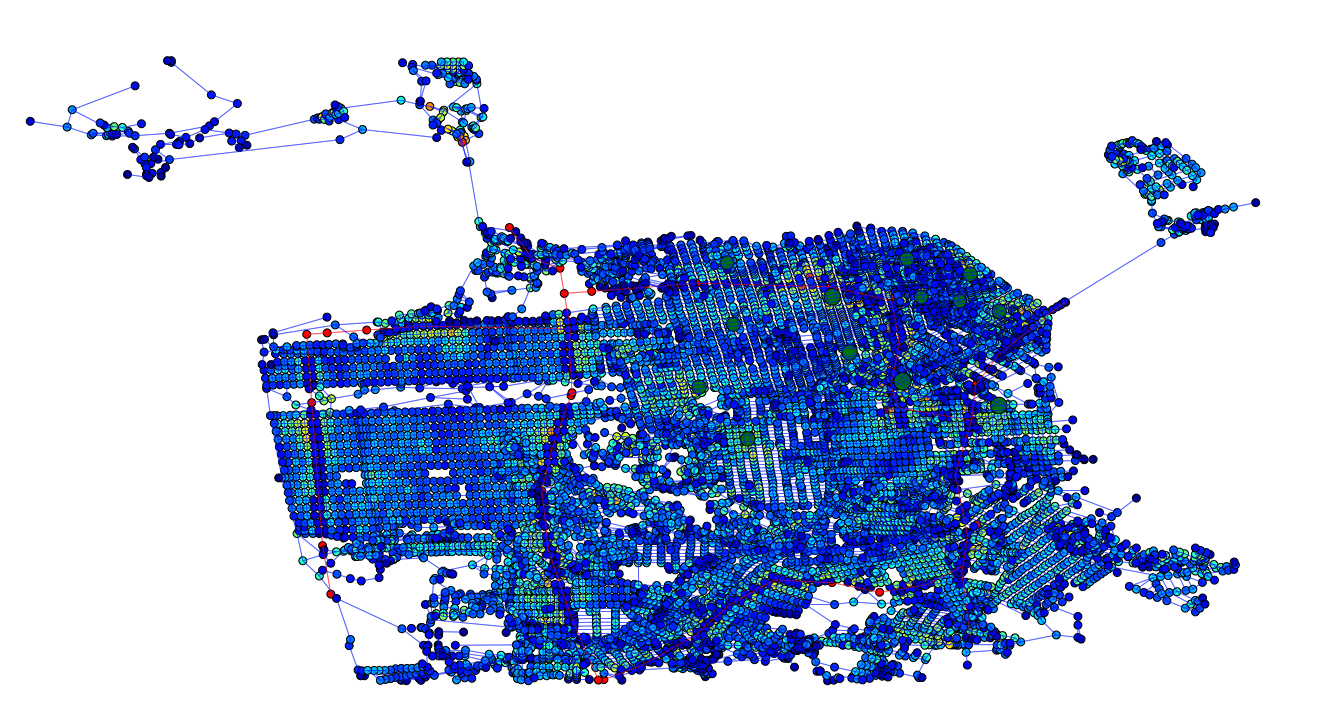
\includegraphics[width=8cm,height=5cm]{../figs/f1}\\
% \end{figure}
Note that this shows several features that we think prove that our model is a successful representation of traffic. At a high level, we can note that almost all of the bright spots cluster around the business nodes, which we found leads to ``over-capacity'' nodes being in places where there is a high demand to get to a business. We can zoom in on various locations to prove that this is a valid representation of traffic. This next image zooms in on the area near the Golden Gate Bridge, notorious for having a significant amount of traffic on commute mornings. \\
 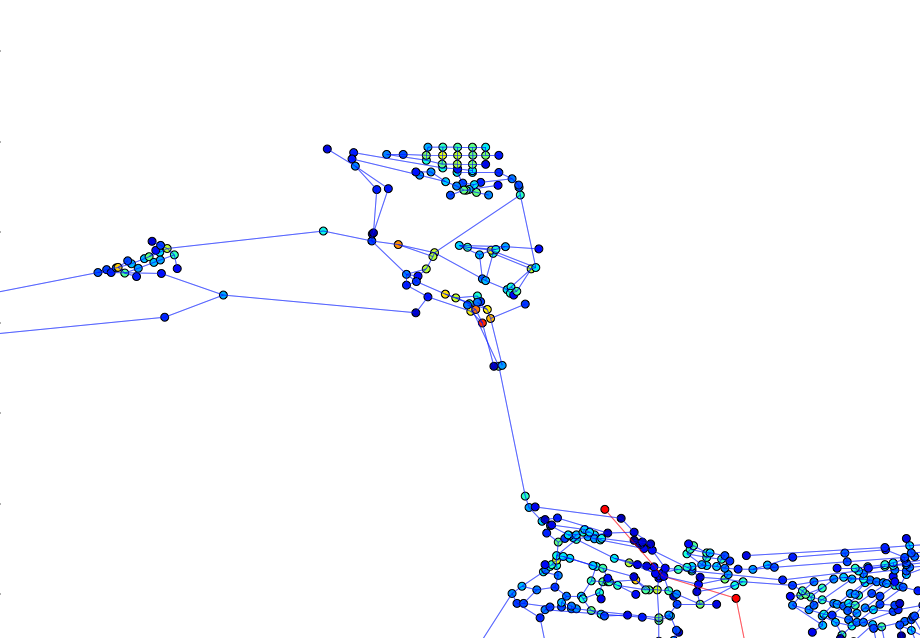
\includegraphics[width=8cm,height=5cm]{../figs/f2} \\
First, we can see several red nodes, which indicate nodes that have gone over capacity. We see on on the bridge, and we see several bright nodes in the area around the bridge. Another example can be seen near the Financial District/Embarcadero, where we had a very large business node (note that this is where several big startups and other companies actually have offices). \\
 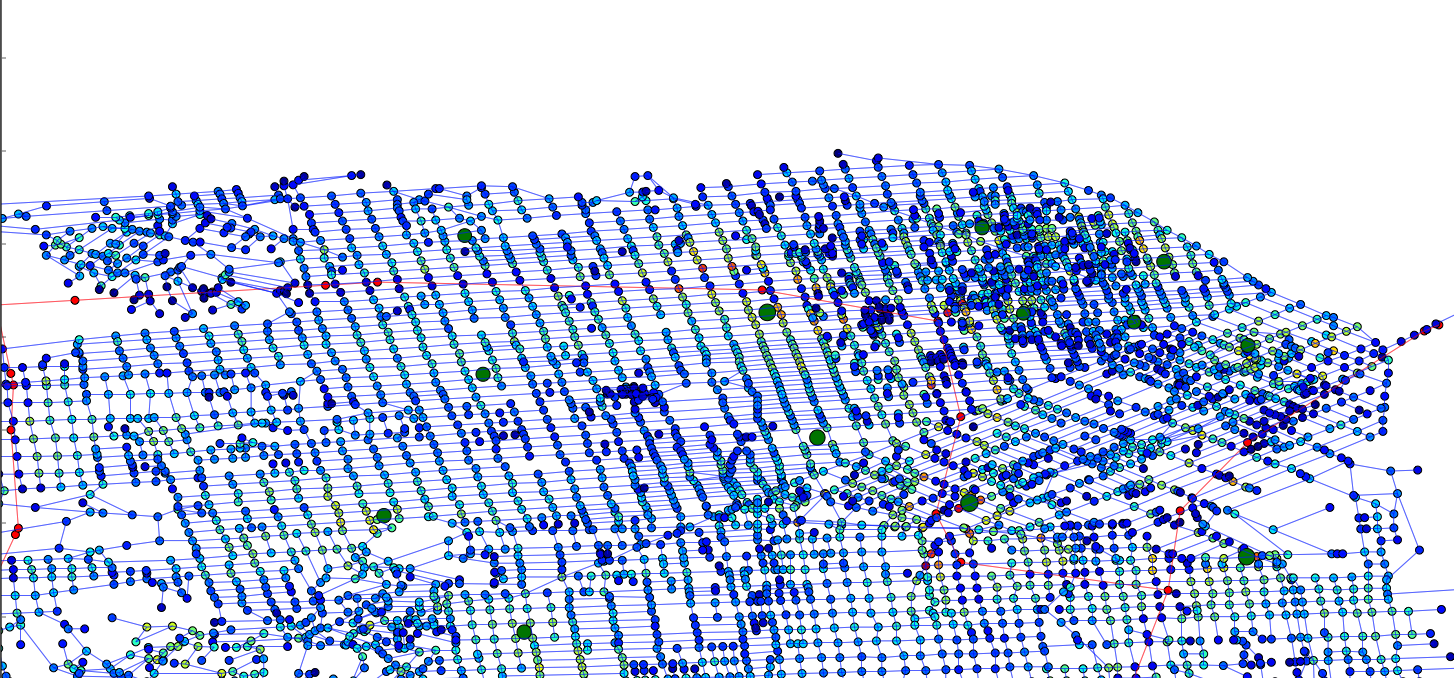
\includegraphics[width=8cm,height=5cm]{../figs/f3} \\
Note that, in this case, the red nodes are actually the highway nodes, but we still see a significant amount of bright spots, particularly near the business nodes, which you can see are the large green nodes.
Finally, and most importantly, we compare the worst capacity-ratio coordinates (the coordinates where there is the most traffic relative to the capacity of the node) returned by the traffic model with an actual average traffic map at peak time from Google Maps: \\
 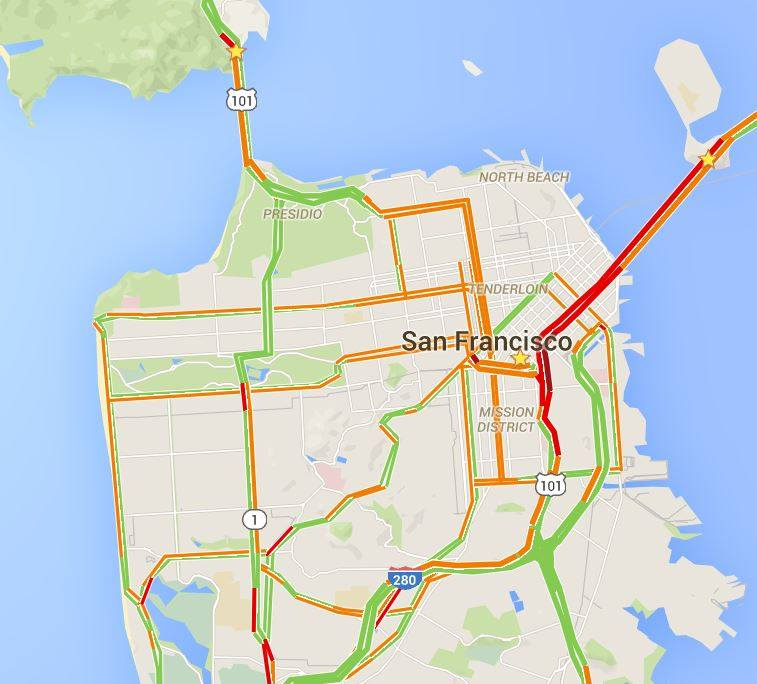
\includegraphics[width=10cm,height=8cm]{../figs/fkey} \\
 The stars are the top 3 points returned by our traffic model, which, at this peak time, look like they have a significant amount of traffic. This is proof that our Markov model indeed accurately represents the traffic. \\
 To run our traffic model, run $\texttt{markov\_map.py}$.
\section{Discussion/Limitations}
Our Markov Chain model for the road San Francisco network and PageRank algorithm as the tool to model traffic flow has various limitations. There are very limited data sets available to that model the road network as graph with nodes and edges – we were very lucky to be able to find a dataset for the San Francisco area.  Therefore, modelling other parts of the country with this technique would be difficult because there simply is not good data available. 

Running the PageRank algorithm with only one crawler also had limitations. Running only a single crawler is not the best model for simulating traffic, a better model would be to run multiple crawlers, one for each car. The one crawler per car model could have potentially been better because transition probabilities between nodes are partially determined by the number of crawlers at a given node. Another issue with the single crawler approach is that the number of iterations of the crawler through the graph must be very high, especially as the graph gets large or else the crawler will not reach sections of the graph. Running PageRank by doing eigenvalue decomposition on a matrix of transition probabilities would have avoided this issue, but this strategy was too computationally intensive. 

One final limitation of the Markov model is that the traffic flow may not meet the condition of a Markov Chain that the next state depends only on the current state and if it does it is very hard to capture all of the information about the current state to allow you to determine the next state.  For example, the transition probabilities of moving from node to node depend on the amount of traffic at a given node, where the node is located, and a variety of other factors. 

Our model produced reasonably good results. You can see from the map below that high probability nodes are clustered around businesses like expected. Also nodes that connect to many other nodes have higher probabilities because the crawler is much more likely to enter those types of nodes and only slightly less likely to leave those nodes.
\end{document}